%%%%%%%%%%%%%%%%%%%%%%%%%%%%%%%%%%%%%%%%%%%%%%%%%
\documentclass[a4paper,11pt]{article}
\pdfoutput=1 % if your are submitting a pdflatex (i.e. if you have
             % images in pdf, png or jpg format)
\usepackage{jheppub} % for details on the use of the package, please
                     % see the JCAP-author-manual
%\usepackage[english]{babel}
\usepackage{amsmath,amssymb,mathtools,tabu}
\usepackage{epsfig,epstopdf}  
\usepackage{graphicx}
\usepackage{slashed}             
\usepackage{url}
\usepackage{color,xcolor}
\usepackage{multirow}
\usepackage{multicol}
\usepackage{placeins}
\usepackage{xspace}
%\usepackage{appendix}
\usepackage{hepnames}
%\usepackage{HEPparticles}
\usepackage{comment} 
\usepackage{tocloft}
\usepackage{ptdr-definitions}
\usepackage{rotating}
%\usepackage{hyperref}
%\usepackage{cite}
\clubpenalty=1000
\widowpenalty=10000
\allowdisplaybreaks

\setlength{\bibsep}{0cm}
\bibpunct{[}{]}{,}{n}{}{,}
%\newcommand{\kt}{\ensuremath{k_{\text{T}}} \xspace}
%\newcommand{\pt}{\ensuremath{p_{\text{T}}} \xspace}
%\newcommand{\GeV}{\ensuremath{\,\text{Ge\hspace{-.08em}V}}\xspace}
%\newcommand{\TeV}{\ensuremath{\,\text{Te\hspace{-.08em}V}}\xspace}
%\newcommand{\ptmiss}{\ensuremath{\pt^\text{miss}}\xspace}
%\newcommand{\ptvecmiss}{\ensuremath{{\vec p}_{\mathrm{T}}^{\kern1pt\text{miss}}}\xspace}
%\newcommand{\fbinv} {\mbox{\ensuremath{\,\text{fb}^{-1}}}\xspace}
\newcommand{\Wprime}{\PWpr\xspace}

\newcommand{\Pb}{{{\Pqb}}\xspace}
\newcommand{\Pt}{{{\Pqt}}\xspace}
\newcommand{\Ps}{{{\Pqs}}\xspace}
\newcommand{\Pc}{{{\Pqc}}\xspace}
\newcommand{\Pd}{{{\Pqd}}\xspace}
\newcommand{\Pu}{{{\Pqu}}\xspace}
\newcommand{\PAb}{{{{\Paqb}}}\xspace}
\newcommand{\PAt}{{{{\Paqt}}}\xspace}
\newcommand{\PAs}{{{{\Paqs}}}\xspace}
\newcommand{\PAc}{{{{\Paqc}}}\xspace}
\newcommand{\PAd}{{{{\Paqd}}}\xspace}
\newcommand{\PAu}{{{{\Paqu}}}\xspace}

%\renewcommand{\PV}{{\ensuremath{{V}}}\xspace}
\renewcommand{\PV}{{{{V}}}\xspace}
%\providecommand{\PV}{{V}\Xspace} % generic vector boson

\newcommand{\VH}{{{\PV}{\PH}}\xspace}


%%%%%%%%%%%%%%%%%%%%%%%% Abstract %%%%%%%%%%%%%%%%%%%%%%%%%%


\begin{document}
\title{SMEFT analysis in Higgs-strahlung}

\author[a]{Suman Chatterjee,}
\emailAdd{suman.chatterjee@oeaw.ac.at}

\affiliation[a]{Institute of High Energy Physics of the Austrian Academy of Sciences (HEPHY)}

%\maketitle

\section*{Project description}

\tableofcontents

\newpage

%------------------------------------------------
\section{Science}\label{sec:sciience}

The large hadron collider (LHC) at CERN has provided a large volume of data till 2018
and is expected to deliver a larger amount of data in the near future
to be compared with theoretical predictions. 
During the Run~2 (2015--2018) era of LHC, CMS experiment~\cite{CMS_ex} has collected proton-proton collision data corresponding to an integrated luminosity of $\sim 140\fbinv$ corresponding to $\sim 10^{16}$ collisions and has been performing an extensive set of analyses to extract the maximum information from those.
A few key milestones LHC reached in last ten years are the following:
\begin{itemize}
\item Discovery of Higgs boson (\PH) in 2012~\cite{Aad:2012tfa,Chatrchyan:2012ufa} resulting in the completion of the standard model (SM) of particle physics. 
This is followed by precision measurements of Higgs boson properties, such as mass~\cite{CMS:2017dib,CMS:2020xrn}, CP nature~\cite{CMS:2019jdw,CMS:2020cga}, coupling to Gauge bosons, third-generation fermions, and second-generation leptons~\cite{CMS-PAS-HIG-19-005}, among others.
\item Precision measurements of processes involving electroweak Gauge bosons (\PW, \PZ, \Pgg), light- and heavy-flavor quarks (\Pu, \Pd, \Ps, \Pc, \Pb, \Pt), gluons (\Pg).
\item Discovery of processes not observed previously in colliders, such as light-by-light scattering~\cite{CMS:2018erd}, single-production of a top quark in association with a \PZ boson~\cite{CMS:2018sgc}, vector boson scattering~\cite{CMS:2017fhs}, among others.
\item Constraining a large region of parameter space in models beyond the SM (BSM) constructed with extended symmetries 
constructed to explain several observed phenomena and to provide an explanation of theoretical quests.
%, including the indications for the existence of dark matter, the origin of nonzero neutrino masses, and the baryon asymmetry of the universe and/or to provide an explanation of the fine tuning required for the insensitivity of the Higgs boson mass to quantum corrections.
\end{itemize}


The lack of a smoking gun evidence of BSM physics predicting new particles within the LHC energy range has motivated the particle physicists to look for subtle deviations in measured distributions of observables from the SM predictions and by systematic field-theoretic extension of the SM Lagrangian adding higher-dimensional operators~\cite{Grinstein:1991cd,Chiu:2007dg,Passarino:2016pzb}.
Higher-dimensional operators, in general, modify the couplings between different particles and result to a smooth change in the shape of particular distributions as compared to SM predictions in precision measurements. 
Precision measurement of Higgs boson couplings, particularly to the vector bosons (\PV), is extremely important in pinning down the structure of the extended SM Lagrangian. 
For example, the existence of a heavy Gauge boson of mass beyond the LHC reach can manifest itself modifying {\PH}-{\PV} couplings~\cite{Appelquist:1974tg}. 
The second most dominant mechanism of Higgs boson production at LHC is in association with a vector boson, referred to as \VH production, which involves a $s$--channel vector boson. 
The \VH production with \PV decaying to leptons is an ideal place to probe \PH in its dominant decay mode to a pair of \Pb quarks as the leptons can be used to select the targeted events and also to reduce the multijet background from quantum chromodynamics (QCD) interaction.
The production of vector boson from quark-antiquark annihilation and the decay of \PH to a pair of \Pb quarks are sensitive to the footprint of new physics at respective vertices, namely vector couplings and Gauge couplings at \VH production and Yukawa coupling in $\PH \to \Pb \PAb$ decay. 
A number of such couplings involving the Higgs boson can be directly probed for the first time at LHC~\cite{Gupta:2014rxa}.
The rest of the couplings, which could have left signatures in earlier experiments like LEP, can also be probed with better accuracy at LHC because of the increase of their impact with energy~\cite{Ellis:2014jta,Grojean:2018dqj}.


The coupling measurements can already be performed with Run~2 LHC data. With the addition of $\sim 160\fbinv$ data to be delivered by LHC in Run~3 (2022--2024), these measurements are expected to have a significant leap in precision.
Therefore, I propose performing an extensive measurement of the couplings relevant in \VH production, where \PV decays leptonically and \PH decays to a pair of \Pb quarks, using differential distributions of a number of observables, some of which have not been measured before.


\section{Research hypothesis}
\label{sec:research_hypo}

\subsection{Effective field theory couplings in \PV($\to$ \Pl\Pl)\PH($\to$ \Pb \PAb) production}

Standard model effective field theory (SMEFT), a generalized extension of the SM, consists of all the possible operators of dimensions greater than four, satisfying the symmetries in SM~\cite{Jenkins:2013zja,Alonso:2013hga,Jenkins:2013wua,Englert:2014cva,Brivio:2017vri}. 
\begin{equation}
\mathcal{L}_{\text{SMEFT}} = \mathcal{L}_{\text{SM}} +  {\sum}_{i} \frac{\text{c}_\text{i}^{\left(5\right)}}{\Lambda} \mathcal{L}_{5}^{i} + {\sum}_{i} \frac{\text{c}_\text{i}^{\left(6\right)}}{{\Lambda}^{2}} \mathcal{L}_{6}^{i} + ...
\label{Eq:SMEFT}
\end{equation}
In Eq.~\eqref{Eq:SMEFT}, $\Lambda$ denotes the cut-off scale which sets an upper limit of the validity of the theory, $\text{c}$'s represent dimensionless numbers, referred to as Wilson coefficients, capturing short-range physics at an energy scale above $\Lambda$, and $\mathcal{L}_{5,6}$ are the operators at dimension-5 and -6, respectively.
The only possible operator at dimension-5, known as Weinberg operator~\cite{PhysRevLett.43.1566}, violates the lepton number conservation and generates Majorana mass to neutrinos~\cite{Bonnet:2009ej}; 
the smallness of neutrino mass points to the relevance of this operator only at energy much higher than that relevant for LHC physics. 
%Number of independent real parameters to describe Wilson coefficients at dimension-6 is known to be 2599~\cit{Alonso:2013hga}, 
The number of independent dimension-6 operators that do not violate baryon and lepton number is known to be 2499,
which can be brought down to 76 assuming the maximum flavor symmetry, $U(3)^5$, 
thereby ignoring differences between different fermion generations
~\cite{Alonso:2013hga}.
The complete set of non-redundant operators at  dimension-6, except for the Hermitian conjugates, written for the first time in 2010 forms the so-called Warsaw basis~\cite{Grzadkowski:2010es}. 
SMEFT operators at dimension-6 modify the production and decay kinematics of the Higgs boson in \VH production compared with those predicted by the SM, which results in differences in shapes of numerous observables constructed using the particles measured in the experiment~\cite{Hagiwara:1993qt,Ellis:2014dva,Murphy:2017omb,Baglio:2020oqu}. 

List of dimension-6 operators in the Warsaw basis that affects the \VH production are listed in Table~\ref{Tab:Operators}.
\begin{table}[t]
\small
\centering
\caption{
Dimension-6 operators in the Warsaw basis affecting the \VH production. %production of Higgs boson in association with a vector boson.
}
\begin{tabular}{c}
\begin{tabular}{c|c}
%\hline
&\\
                ${\cal O}^{(1)}_{Hq}=i H^\dagger  \overleftrightarrow{D}_\mu H \bar{q}   \gamma^\mu q$&${\cal O}_{HWB}=  H^\dagger \sigma^a H W^a_{\mu\nu}B^{\mu\nu}$ \\
\rule{0pt}{4ex} ${\cal O}^{(3)}_{Hq}=i H^\dagger \sigma^a \overleftrightarrow{D}_\mu H \bar{q}  \sigma^a \gamma^\mu q$ &${\cal O}_{H\tilde{W}B}=  H^\dagger \sigma^a H W^a_{\mu\nu}\tilde{B}^{\mu\nu}$\\
\rule{0pt}{4ex} ${\cal O}_{Hu}=i H^\dagger \overleftrightarrow{D}_\mu H \bar{u}_R  \gamma^\mu u_R$&${\cal O}_{H{W}}= |H|^2 W_{\mu\nu}{W}^{\mu\nu}$\\
\rule{0pt}{4ex} ${\cal O}_{Hd}=i H^\dagger \overleftrightarrow{D}_\mu H \bar{d}_R  \gamma^\mu d_R$&${\cal O}_{H\tilde{W}}= |H|^2 W^a_{\mu\nu}\tilde{W}^{a \mu\nu}$\\
\rule{0pt}{4ex} ${\cal O}_{HD}=(H^\dagger  {D}_\mu H)^*(H^\dagger  {D}_\mu H)$& ${\cal O}_{HB}= |H|^2 B_{\mu\nu}B^{\mu\nu}$\\
\rule{0pt}{4ex} ${\cal O}_{H\square}=(H^\dagger H) \square (H^\dagger H)$& ${\cal O}_{H\tilde{B}}= |H|^2 B_{\mu\nu}\tilde{B}^{\mu\nu}$\\
&\\
%\hline
 \end{tabular}
\end{tabular}
\label{Tab:Operators}
\end{table}
First four operators in the left column of Table~\ref{Tab:Operators} introduce 4-point interactions, shown in Fig.~\ref{fig:Feynman_digarams} (left). 
The same operators along with ${\cal O}_{HD}$ and ${\cal O}_{HWB}$ affect the coupling of \PV to fermions, shown in Fig.~\ref{fig:Feynman_digarams} (middle). 
The remaining operators modifies \PH--\PV coupling as shown in Fig.~\ref{fig:Feynman_digarams} (right). 
\begin{figure*}[hbtp]
\begin{center}
\includegraphics[width=0.321\textwidth]{Figures/Feynman_diagrams/ffVh.png}
\includegraphics[width=0.321\textwidth]{Figures/Feynman_diagrams/Vff.png}
\includegraphics[width=0.321\textwidth]{Figures/Feynman_diagrams/hVV.png}
\end{center}
\caption{
Fragments of the Feynman diagram for \VH production sensitive to different dimension-6 operators.
}
\label{fig:Feynman_digarams}
\end{figure*}

\subsection{Direct measurements of SMEFT couplings in \PV($\to \Pl \Pl $) \PH ($\to \Pb \PAb$)}

SMEFT parameters can, in general, be constrained using data from the previous low-energy experiments by replacing \PH by its vacuum expectation value ($v$) in operators in Table~\ref{Tab:Operators}. For a majority of the operators at work here, which are of the form ${\PH}^2\mathcal{L}_{\text{SM}}$,
this just corresponds to a shift of the parameters in SM Lagrangian. 
Therefore, those can be probed directly for the first time at LHC.

Now, the operators at Table~\ref{Tab:Operators} can also be constrained using the existing measurements in Higgs sector at LHC~\cite{CMS-PAS-HIG-19-005,ATLAS:2020fcp,ATLAS:2020jwz}. 
However, this methodology assumes that all the object and event selection conditions have the same efficiency and acceptance for the SM and SMEFT operators, 
which is known to be not the case always. 
Also, as will be shown in Sec.~\ref{sec:method}, some important effects can be lost in traditional measurements of kinematic variables. 
Therefore, it is necessary to construct a set of observables that can extract telltale signatures of EFT operators without any loss of information. 
Also, the impact of all the conditions applied at the analysis level needs to be checked for the operators involved. 
These goals can only be achieved in a dedicated measurement as proposed here.

\section{Objectives}
\label{sec:objective}

The goal of this proposal is to probe the operators listed in Table~\ref{Tab:Operators} in \VH production as precisely as possible.
Dependence of the production cross section of \VH process on the Wilson coefficients corresponding to ${\cal O}^{(3)}_{Hq}$, ${\cal O}_{HW}$, and ${\cal O}_{HWB}$, denoted as cpq3i and cpW, respectively, in different regions in vector boson transverse momentum (\pt) are shown in Fig.~\ref{fig:LHE_WZH} for $\PW\PH$ and $\PZ\PH$ productions. 
\begin{figure*}[hbtp]
\begin{center}
\includegraphics[width=0.321\textwidth]{Figures/LHE/WH/Canv_cpq3i.png}
\includegraphics[width=0.321\textwidth]{Figures/LHE/WH/Canv_cpW.png}
\includegraphics[width=0.321\textwidth]{Figures/LHE/WH/Canv_cpWB.png}

\includegraphics[width=0.321\textwidth]{Figures/LHE/ZH/Canv_cpq3i.png}
\includegraphics[width=0.321\textwidth]{Figures/LHE/ZH/Canv_cpW.png}
\includegraphics[width=0.321\textwidth]{Figures/LHE/ZH/Canv_cpWB.png}
\end{center}
\caption{
Variation of cross section of $\PW\PH$ (top) and $\PZ\PH$ (bottom) productions relative to the SM prediction as a function of Wilson coefficients corresponding to ${\cal O}^{(3)}_{Hq}$ (left), ${\cal O}_{HW}$ (middle), and ${\cal O}_{HWB}$ (right) in five regions of $\PW$ and $\PZ$ boson {\pt}, respectively.
}
\label{fig:LHE_WZH}
\end{figure*}
%Figs.~\ref{fig:LHE_WH} and~\ref{fig:LHE_ZH} exhibit the following features: ${\cal O}^{(3)}_{Hq}$ induces a rapid
These three operators, along with their corresponding CP-odd counterparts, and ${\cal O}_{HD}$ , ${\cal O}_{H\square}$  affect both $\PW\PH$ and $\PZ\PH$ productions, whereas ${\cal O}^{(1)}_{Hq}$, ${\cal O}_{Hu}$, ${\cal O}_{Hd}$, ${\cal O}_{HB}$, and ${\cal O}_{H\tilde{B}}$ affect only $\PZ\PH$ production 
because of the helicity structure involved in $\Pquark\APquark \to \PZ\text{,}\PW$ interaction.
The SM cross section for $\PW\PH$ production, where $\PW$ decays to either a muon or an electron is roughly 20 times larger than $\PZ\PH$ production, where $\PZ$ decays to a pair of electrons and muons, 
so the former results in better statistical precision in the measurements.
Therefore, measurement of couplings in both $\PW\PH$ and $\PZ\PH$ processes is necessary to probe the complete set of operators relevant to \VH production as also shown in Ref.~\cite{Banerjee:2019twi}.
A preliminary study to test the sensitivity to certain operators is presented in Sec.~\ref{sec:method}. 


\section{Scientific originality}

Although the SMEFT operators can be indirectly probed using results from the previous experiments, 
LHC gives a unique opportunity to directly measure a number of SMEFT operators, particularly those involving the Higgs field~\cite{Elias-Miro:2013mua,Gupta:2014rxa}. 
So far, there exist very few measurements where all the efficiency and acceptance effects of object and event selection conditions are taken into account, and complete information contained in an event is used.
The proposed measurement will extend the scope of probing new physics scenarios using previously unexplored angular observables.% discussed in Sec.~\ref{sec:method}.
A list of new things aimed to be developed and applied during the proposed measurements are the following:
\begin{itemize}

\item The complete set of event information, parameterized by kinematic and angular variables, will be used for the first time in \VH production followed by \PV $\to$ \Pl \Pl and $\PH \to \Pb \PAb$. 
The newly proposed methods which can be applied in this context are 
'method of moments'~\cite{Banerjee:2019twi,Banerjee:2020vtm} and 
boosted information tree~\cite{Chatterjee:2021nms}.
The latter one is developed by the group where the proposer belongs to. 
Development of the methods and applying those in a CMS measurement by the same group will greatly accelerate the preparation of the results. 

\item Deep neural network based algorithms are used to identify \PH decaying to a pair of \Pb quarks, and efficiency of the tagger is conventionally measured in data and simulation in $\Pg \to \Pb \PAb$ process. 
However, \Pg and \PH are very different in mass, spin, and color properties. During the proposed work, an effort will be pursued to improve the calibration of the tagger, 
particularly using $\PZ \to \Pb \PAb$ decay.

\end{itemize}


\section{Relevance to the research field}

The idea of EFT has prevailed in the context of particle physics since as late as the 1930s with the Fermi theory of beta decay~\cite{Fermi:1934hr} and Yukawa theory of meson exchange~\cite{Yukawa:1935xg}.
Those guided the particle physics community through a long and adventurous journey, 
which has led to the development of the SM in its present form. 
The lack of convincing hints of new physics at LHC has automatically shifted the focus of the community's interests towards EFT as the future step~\cite{Ellis:2018gqa,Ellis:2020unq,Ethier:2021bye} 
and measurements of higher-dimensional operators has started to take the center stage of LHC physics program~\cite{CMS:2021nnc,CMS:2021aly,CMS:2021gme}.
The interests in both theory and experiment communities are growing at an increasing rate, 
which can be gauged by the formation of the LHC EFT working group~\cite{LHC_EFT_WG} and the conduction of a series of lectures under the `All things EFT' forum~\cite{All_EFT}. 
So, it is a call of time to perform dedicated EFT measurements at LHC.
The proposed measurement not only probes a set of unique EFT operators in the Higgs sector but also complements the ongoing measurements of EFT operators in the area of electroweak bosons and top quark and enhances the physics potential of LHC experiments on a broad scale. 
For example, measurements of the vector couplings involving light quarks nicely complement the measurement of the similar couplings involving top quarks and they together can probe the flavor universality in quark sector.
The results of these measurements will constitute the output from LHC to be used in a global EFT fit, combining results of many different experiments.
Therefore, it is high time for the group to perform the proposed measurement and strengthen its position in the international community. 

\section{Method}
\label{sec:method}

Achieving goals in time requires setting up a concrete plan in advance. 
The target is to utilize the data available for physics analysis from LHC Run~2, corresponding to an integrated luminosity of 139\fbinv at $\sqrt{s}=13\TeV$, and also the data to be recorded during LHC Run~3, which is expected to be $\sim 160\fbinv$ at around the same $\sqrt{s}$. 
With $\sim 45\%$ of the total dataset already in the disk, the strategy is to finalize the analysis procedures with Run~2 data and publish the first set of results, which will be followed by a final paper using data to be collected by 2024. 

In the following, a brief discussion of the analysis strategy to achieve goals mentioned in Sec.~\ref{sec:objective} is made. The feasibility study reported here is performed focusing primarily on $\PW\PH$ production, 
nevertheless, also some additional features available in $\PZ\PH$ are mentioned. 

\subsection{Final states and observables}

The following final states are considered.
\begin{itemize}
\item $\PW\left(\to \Pl \Pgn \right) \PH \left(\to \Pb \PAb \right)$
\item $\PZ\left(\to {\Pl}^{+} {\Pl}^{-} \right) \PH \left(\to \Pb \PAb \right)$
\end{itemize}
%Since $\PH \to \Pb \PAb$ has the largest branching ratio, its use enables to improves the statistics of the analyzed event sample. 
%Leptonic decay of the vector boson helps to get rid of the background from the multijet production in QCD, which is the dominant background in most of the hadronic final states. 

As mentioned in Sec.~\ref{sec:research_hypo} and~\ref{sec:objective}, operators listed in Table.~\ref{Tab:Operators} introduce an energy growth, which will be visible in distributions of traditional kinematic observables, like \pt of vector boson or Higgs boson. 
However, only a few kinematic observables are not enough to disentangle the effects of a relatively large number of SMEFT operators. 
A systematic analysis of \VH production process starting from helicity amplitudes, 
as performed in Ref.~\cite{Banerjee:2019twi}, 
enables to learn about angular variables, shown in Fig.~\ref{fig:HelicityFrame}, 
which are complementary to the kinematic variables exhibiting energy growth, and 
they together fully characterize the event structure.
\begin{figure*}[hbtp]
\begin{center}
\includegraphics[width=0.75\textwidth]{Figures/LHE/TheThreeAnglesVh.pdf}
\end{center}
\caption{
Pictorial depiction of the angles describing the final state in \PV($\to \Pl \Pl$\PH($\to Pb PAb$) production.
}
\label{fig:HelicityFrame}
\end{figure*}
The helicity amplitudes corresponding to longitudinal and transverse polarizations of the vector boson contributing to the full amplitude of \VH production are affected differently by the operators involved.
Thus, rich information about the event structure can be obtained by a joint analysis of kinematic and angular variables.
In a traditional cross section measurement integrated over angular variables, 
effects of the interference between helicity amplitudes are lost, and those can be resurrected using the angular information~\cite{Panico:2017frx}.

\begin{comment}
once calculates helicity amplitudes in \VH center-of-mass frame and the cross section has the following form:
\begin{equation}
{\sigma}_{\VH} (\hat{s},\Theta,\theta,\phi) = {\sum}_{i=1}^{9} a_{i}(\hat{s}) f_{i}(\Theta,\theta,\phi)	\ .
\label{Eq:Xsection}
 \end{equation}  
In Eq.~\eqref{Eq:Xsection}, $a_{i}$, parameterizing the dependence of Wilson coefficient and energy transfer $\hat{s}$, are known as angular moments and $f_{i}$ encapsulates the dependency on the angles $\Theta,\theta,\phi$ defined in Fig.~\ref{fig:HelicityFrame}.
\begin{figure*}[hbtp]
\begin{center}
\includegraphics[width=0.75\textwidth]{Figures/LHE/TheThreeAnglesVh.pdf}
\end{center}
\caption{
Definition
}
\label{fig:HelicityFrame}
\end{figure*}
The functions $a$ and $f$ contain the complete information of how \VH production is affected by dimension-6 SMEFT operators and their forms can be found in Ref.~\cite{Banerjee:2019twi}. 
However, the absence of knowledge about the directions of incoming quark and anti-quark leads to the vanishing of three angular moments. Among the remaining six angular moments, two correspond to the case where the vector boson is either transversely or longitudinally polarized, and the remaining four correspond to the interference of two amplitudes with different polarizations of the vector boson. An inclusive measurement over all the angles lead to the vanishing of the later four angular moments, thus a loss of information about the event structure. 

In this proposal, we target to use complementary kinematic and angular observables in \VH process and probe the SMEFT operators at work.


We consider the final states as follows.
\begin{itemize}
\item $\PW\left(\to \Pl \Pgn \right) \PH \left(\to \Pb \PAb \right)$
\item $\PZ\left(\to \Pl \Pl \right) \PH \left(\to \Pb \PAb \right)$
\end{itemize}
Since $\PH \to \Pb \PAb$ has the largest branching ratio, its use enables to improves the statistics of the analyzed event sample. 
Leptonic decay of the vector boson helps to get rid of the background from the multijet production in QCD, which is the dominant background in most of the hadronic final states. 
The lepton(s) from the vector boson also helps to trigger the events. The process $\PZ\left(\to \Pgn \Pgn \right) \PH \left(\to \Pb \PAb \right)$ is ignored here since we need the lepton directions to construct the angular variables.

\end{comment}

\subsection{Event selection and categorization}

Lepton(s) from \PW or \PZ boson is (are) used to trigger the events to be analyzed. 
CMS trigger system, developed centrally within the Collaboration, is used to select events with at least one lepton (\Pl) satisfying a threshold in {\pt}.
At very high \pt of the vector boson, backup triggers requiring a considerable hadronic activity can be used particularly for the final state with electron(s). 
Measurement of efficiency of the triggers both data and simulation is an essential step of the analysis to understand the modeling of the selected events in data by simulation.
Tag-and-probe method in $\PZ \to {\Pl}^{+} {\Pl}^{-}$ events will be used to measure the trigger efficiencies. Corrections will be derived in simulation to match the trigger efficiency in data.
For the feasibility study, it is assumed that trigger efficiencies are the same in data and simulation.

An event to be selected as a $\PW\PH$ candidate event is required to have an electron or a muon with \pt$>32$ and $>25$\GeV, respectively passing the identification conditions corresponding to 90 and 95\% efficiency for genuine electron and muon, respectively. 
The four-momentum of neutrino is reconstructed using the missing transverse momentum vector (\ptvecmiss) and assuming that the invariant mass of neutrino and lepton system is always the value of $\PW$ boson mass provided by the particle data group. 
This will be discussed further in Sec.~\ref{sec:neu_reco}. 
The \PW boson reconstructed from lepton and neutrino momenta is required to satisfy $\pt > 150$\GeV, which brings down the contamination from multijet production to a negligible extent.
The lepton and \ptvecmiss are required to satisfy $\Delta \phi > 2$ radian, where $\Delta \phi$ is the angular separation in the plane transverse to the collision axis.
The event is also required not to contain any additional electrons or muons with $\pt>25$\GeV satisfying the identification requirement specified earlier.

The selected events are further categorized into regions depending on the jet system. 
If \PH has a large \pt, its decay products are merged into a large-sized jet. 
In this case, referred to as boosted topology, 
jets reconstructed using anti-\kt algorithm with distance parameter 0.8, referred to as AK$8$ jets are used to identify \PH.
Otherwise, \PH is reconstructed using AK$4$ jets initiated by its daughter \Pb quarks; 
this is referred to as resolved topology.
In CMS, DNN-based taggers, henceforth referred to as DeepJet and DeepAK8 taggers, are used to identify AK4 jets initiated by \Pb quarks~\cite{Bols:2020bkb} and AK8 jets initiated by \PH decaying to a pair of \Pb quarks~\cite{Sirunyan:2020lcu}, respectively.
DeepAK8 tagger actually provides multiple outputs that correspond to the probability of AK8 originating from top quark, \PW boson, light quark or gluon, etc.; this information is also used later.

In resolved topology, the system of two AK4 jets with highest \Pb tagging scores, referred to as b1 and b2, is taken as the \PH candidate, whereas the AK8 jet with the highest \PH tagging score is taken as the \PH candidate in boosted topology.
Signal region (SR), enriched by $\PW\left(\to \Pl \Pgn \right) \PH \left(\to \Pb \PAb \right)$ events, is constructed using the conditions listed in Table~\ref{Tab:Regions}.
\begin{table}[t]
\small
\centering
\caption{
Selection conditions targeted for $\PW\PH$ events.
}
\begin{tabular}{c}
\\
\begin{comment}
Exactly one \Pmu (\Pe) with $\pt>24(32)\GeV$ and $|\eta|<2.5$ \\
No additional \Pmu or \Pe with $\pt>25\GeV$ and $|\eta|<2.5$ \\
$\Delta\phi(\Pl,\ptvecmiss)>\pi$ ($\ptvecmiss$ is the missing transverse momentum vector) \\
Neutrino momentum computed using $|\ptvecmiss|$ and \PW mass ($=80.4\GeV$) \\
${\pt}^{\PW} > 75\GeV$ \\
\\
Higgs boson candidate\\
\hline
\end{comment}
\end{tabular}
\begin{tabular}{m{8cm} | m{8cm}}
Resolved category & Boosted category \\
\hline
%Two AK4 jets with highest \Pbottom tagging score (say, b1, b2) & AK8 jet with the highest \PHiggs tagging score \\
$>=$2 b-tagged AK$4$ jets ($\pt>30\GeV$, $|\eta|<2.5$) & $>=1$ AK8 jets ($\pt>250\GeV$, $|\eta|<2.5$)\\ 
B tagging score of b1 $>$ btag$^{\text{cut}}_{\text{max}}$ & \PH tagging score of \PH $>$ Htag$^{\text{cut}}$\\
B tagging score of b2 $>$ btag$^{\text{cut}}_{\text{min}}$ & \\
$<2$ additional AK4 jets & No. of b-tagged AK4 jets outside \PH $=0$  \\
$M(b1+b2) \epsilon [90,150]\GeV$ & Soft-drop mass of \PH $\epsilon [90,150]\GeV$ \\
\end{tabular}
\label{Tab:Regions}
\end{table}
In Table~\ref{Tab:Regions}, btag$^{\text{cut}}_{\text{max}}$ and btag$^{\text{cut}}_{\text{min}}$ represent thresholds on DeepJet score corresponding to 1\% and 10\% mistag rate for light quark or gluon jets, respectively, and Htag$^{\text{cut}}$ corresponds to threshold on \PH tagging score corresponding to 1\% mistag rate for the same background.
Changing the conditions on variables in  Table~\ref{Tab:Regions}, one also gets control regions (CRs) enriched by different background processes. 
For example, requiring no. of additional jets (no. of b-tagged jets outside the \PH candidate) $\geq 2$ in the resolved (boosted) category enables to select a phase space enriched by the events with pair production of top quarks ($\Pt\PAt$).
The phase space one gets inverting the mass condition on the \PH candidate in the SR is dominated by vector boson in association with jets initiated by $\Pb$ and $\Pc$ quarks (${\PW}+\Pb/\Pc$). 
Finally, events failing the condition of the presence of two b-tagged AK4 jets (one Higgs-tagged AK8 jet) are dominated by the production of vector boson in association with light quark jets (${\PW}+$j).
These CRs can be used to measure the corresponding backgrounds and validate those using data.

Distribution of \PW boson \pt in resolved and boosted categories of the SR are shown in Fig.~\ref{fig:RECO_Vpt_WH}, where the change in $\PW\PH$ signal with the operators ${\cal O}^{(3)}_{Hq}$ and ${\cal O}_{HW}$ turned on with the corresponding Wilson coefficients set to 1 are also overlaid. 
\begin{figure*}[hbtp]
\begin{center}
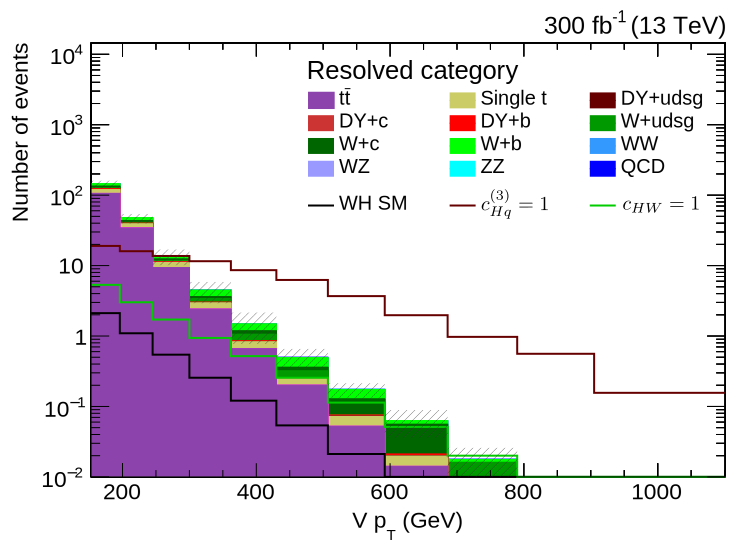
\includegraphics[width=0.45\textwidth]{Figures/RECO/Plot_Resolved_SR_V_pt.png}
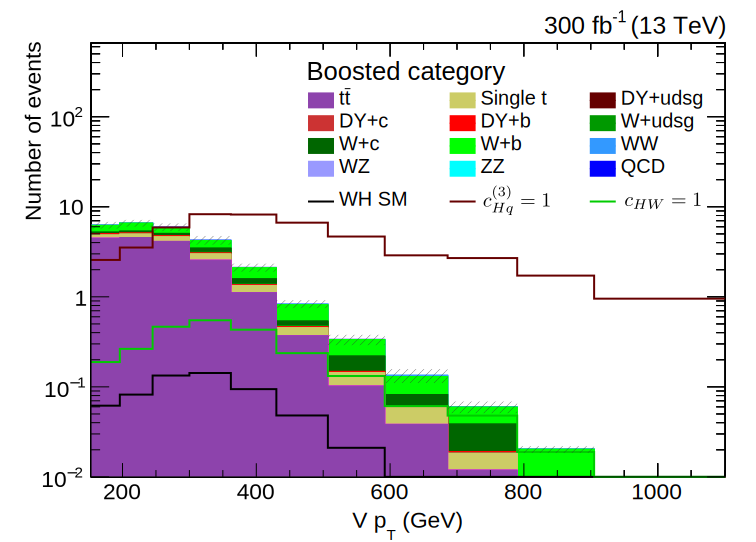
\includegraphics[width=0.45\textwidth]{Figures/RECO/Plot_Boosted_SR_V_pt.png}
\end{center}
\caption{
Distribution of \PW boson \pt in resolved (left) and boosted (left) categories of the SR. Impact of systematic uncertainties on jet energy scale and resolution, correction factor used to match the b-tagging and Higgs-tagging efficiencies in data and simulation are shown in the bottom panel.
}
\label{fig:RECO_Vpt_WH}
\end{figure*}
Fig.~\ref{fig:RECO_Vpt_WH} shows that the main backgrounds to $\PW\PH$ signal are events from $\Pt\PAt$ and ${\PW}+\Pb/\Pc$ productions.

The shape of the distribution of angular variables is also sensitive to some of the dimension-6 operators. As shown in Fig.~\ref{fig:angles}, 
the SM production dominated by longitudinal polarization of \PW boson has some differences w.r.t the case when ${\cal O}_{HW}$  operator is turned on since it causes interference between amplitudes with longitudinal and transverse polarizations of \PW boson. 
Variable $\phi$, on the other hand, is very sensitive to the CP-nature of the operators, and the difference in its modulation between CP-even and CP-odd operators is clearly visible in $\PZ\PH$ production. CP-sensitivity in $\phi$ is reduced in $\PW\PH$ production due to the ambiguity in neutrino reconstruction as will be shown in Sec.~\ref{sec:neu_reco} and the impact of other particles in the process on \ptmiss; this needs a dedicated study in future.
\begin{figure*}[hbtp]
\begin{center}
\includegraphics[width=0.45\textwidth]{Figures/RECO/Angle/WH/Boosted_Plot_Theta.png}
\includegraphics[width=0.45\textwidth]{Figures/RECO/Angle/ZH/Boosted_Plot_Theta.png}
\includegraphics[width=0.45\textwidth]{Figures/RECO/CP/WH/Resolved_Plot_phi.png}
\includegraphics[width=0.45\textwidth]{Figures/RECO/CP/ZH/Resolved_Plot_phi.png}
\end{center}
\caption{
Normalized distribution of polar angle $\Theta$ in $\PW\PH$ (top left) and $\PZ\PH$ (top right) productions for $cpW=1$ and SM scenarios in boosted category. 
Normalized distribution of azimuthal angle $\phi$ in  $\PW\PH$ (bottom left) and $\PZ\PH$ (bottom right) productions for $cpW=1$ and $\tilde{cpW}=1$, respectively; SM component is subtracted from in these distributions.
}
\label{fig:angles}
\end{figure*}


\subsection{Neutrino reconstruction}
\label{sec:neu_reco}

In order to reconstruct the momentum of invisible neutrino in $\PW \to \Pl \Pgn$, we assume that the \Pnu is the only source of $\ptvecmiss$ in the event and take its $\pt$ and $\phi$ as the same of \Pnu. 
Finally, we use $\PW$-mass constraint to calculate $\eta$ of \Pnu, denoted as ${\eta}^{\Pgn}$. However, the quadratic nature of mass constraint gives rise to two possible solution for  ${\eta}^{\Pnu}$ as follows.
\begin{equation}
 {\eta}^{\Pnu} = {\eta}^{l} \pm cosh^{-1}(1+{\Delta}^2)	\ ,
\label{Eq:NeuEta}
\end{equation}
where ${\Delta}^2 = \frac{m_W^2 - m_T^2 ({p^l},{p^\text{miss}\xspace})}{2 p_T^{l} p_T^{miss}}$. 
When \PW boson has large \pt, which results to $\Delta << 1$, these two solutions become 
\begin{equation}
{\eta}^{\Pnu} \simeq {\eta}^{l} \pm \sqrt{2}{\Delta} + {\cal{O}} ({\Delta}^3)	\ ,
\label{Eq:NeuEta2}
\end{equation}
In this limit,  the angular variable $\theta$ and $\Theta$ computed with these two solutions converge to the same values, whereas the variable $\phi$ does not. 
It can be shown that $\phi$ computed with two solutions are related by the $\phi_{+} \simeq \pi - \phi_{-}$. This ambiguity is visible in Fig.~\ref{fig:neureco}.
\begin{figure*}[hbtp]
\begin{center}
\includegraphics[width=0.45\textwidth]{Figures/RECO/Resolved_Plot_2D_phi_unweighted.png}
\includegraphics[width=0.45\textwidth]{Figures/RECO/Boosted_Plot_2D_phi_unweighted.png}
\end{center}
\caption{
Correlation between $\phi$ calculated at parton level and detector level in resolved (left) and boosted (right) categories in $\PW\PH$ production.
}
\label{fig:neureco}
\end{figure*}

The ambiguity in $\phi$ reduces the CP-sensitivity in $\PW\PH$ production. A dedicated study needs to be performed to overcome this limitation.


\subsection{Multivariate analysis}

As seen from Fig.~\ref{fig:RECO_Vpt_WH}, the region SR has a large number of background events.
To separate the  $\PW\PH$ signal even more from the background events, particularly due to $\Pt\PAt$ production, 
a multivariate (MVA) discriminator is constructed using a DNN with two fully connected dense layers. 
Input variables to the DNN in the resolved category are listed in Table~\ref{Table:MVA_Vars}.
\begin{table}[t]
\small
\centering
\caption{
Input variables to the DNN designed to separate events from $\PW\PH$ and $\Pt\PAt$ productions.
}
\begin{tabular}{m{7cm}  m{10cm}}
\\
 \pt component of \ptvecmiss & No. of AK4 jets ($\pt>30\GeV$, $|\eta|<2.5$) \\
\pt and $\eta$ of the lepton & B tagging scores of b1 and b2 \\
$\Delta\phi(\Pl,\ptvecmiss)$ & Ratio of the \pt of b1 and b2 \\
No. of additional jets  &  Minimum of the \pt of b1 and b2 \\
Event thrust (see definition in~\cite{CMS:2014tkl}) &  Maximum of the \pt of b1 and b2 \\
Rapidity and mass of \PH candidate & Maximum of relative \pt of the lepton w.r.t. b1 and b2 \\
$\Delta\phi(\PW,\PH)$ & $\Delta\phi(\text{b1},\text{b2})$ \\
\\
\end{tabular}
\label{Table:MVA_Vars}
\end{table}
A similar discriminator is built in the boosted category using the variables in the left column of Table~\ref{Table:MVA_Vars} along with the following variables corresponding to the \PH candidate AK8 jet: 
the output of DeepAK8 taggers quantifying the probability of the jet originated due to top quark, Higgs boson, \PW boson relative to the same originated from a light quark or gluon.
Normalized distributions of MVA discriminators in SM $\PW\PH$ and $\Pt\PAt$ events are shown in Fig.~\ref{fig:MVA}. 
Resistive operator characteristics (ROC) curves are obtained by computing the fraction of signal and background events varying thresholds on the MVA discriminators.
\begin{figure*}[hbtp]
\begin{center}
\includegraphics[width=0.45\textwidth]{Figures/RECO/Plot_WH_MVA_WH_fast_resolved.png}
\includegraphics[width=0.45\textwidth]{Figures/RECO/ROC_plot_TT_MVA_resolved.png}
\includegraphics[width=0.45\textwidth]{Figures/RECO/Plot_WH_MVA_WH_fast_boosted.png}
\includegraphics[width=0.45\textwidth]{Figures/RECO/ROC_plot_TT_MVA_boosted.png}
\end{center}
\caption{
Normalized distributions of the MVA discriminator in signal ($\PW\PH$) and background ($\Pt\PAt$) events (left) and ROC curve characterizing the performance of MVA discriminator (right) in the resolved (top) and boosted (bottom) categories.
}
\label{fig:MVA}
\end{figure*}

\subsection{Sensitivity results}

Although the final condition on the MVA discriminator needs to be optimized, 
we go on checking the sensitivity by choosing a threshold on the MVA discriminator, 
which corresponds to $80\%$ signal efficiency; this corresponds $\sim 30\%$ ($\sim 15\%$) background efficiency in the resolved (boosted) category.
For simplicity, we use the efficiency numbers for different event samples as the first step and perform one-dimensional likelihood scans for two Wilson coefficients corresponding to operators ${\cal O}^{(3)}_{Hq}$ and ${\cal O}_{HW}$, respectively, while setting others to $0$. The results are shown in Fig.~\ref{fig:NLL} for the integrated luminosity of 300\fbinv.
\begin{figure*}[hbtp]
\begin{center}
\includegraphics[width=0.45\textwidth]{Figures/RECO/Full_NLL_WC_cpq3i_fine_300fb_opt1.png}
\includegraphics[width=0.45\textwidth]{Figures/RECO/Full_NLL_WC_cpW_fine_300fb.png}
\end{center}
\caption{
Variation of the profile likelihood ratio $q$ as a function of Wilson coefficients corresponding operators ${\cal O}^{(3)}_{Hq}$ (left) and ${\cal O}_{HW}$ (right) for an integrated luminosity of 300\fbinv.
}
\label{fig:NLL}
\end{figure*}
Fig.~\ref{fig:NLL} shows that a large gain in sensitivity is obtained by adding the boosted category due to the energy growth induced by the operators. 
The preliminary results show that the Wilson coefficient corresponding to ${\cal O}^{(3)}_{Hq}$ can be constrained to percent level and the one corresponding to ${\cal O}_{HW}$ within $\sim [-0.4,0.25]$ at 95\% confidence level. 
An improvement due to a binning in $\phi$ is also observed in the resolved category.
The use of information about all three angles $\Theta$, $\theta$, $\phi$ is expected to result in a large increase in sensitivity.

\subsection{Possible extensions of ideas}

The research plan proposed here can also be extended in multiple directions, such as the following. 

\begin{itemize}

\item The constraints obtained from  the proposed measurements can also be reinterpreted as bounds on new physics models of interest, for example, on models predicting the existence of a \PZprime and \PWprime bosons in $\PZprime \to \PZ \PH$ and $\PWprime \to \PW \PH$ decays, respectively.
Particularly, new physics models with \PZprime is in highlights in recent times to explain the anomalies in the flavor sector. 

\item Here, the proposal is to probe SMEFT operators in \VH production, where \PV decays to leptons. 
But, the methodology developed also holds for hadronically decaying \PV; 
the only bottleneck in the case of {\PV}$ ={\PW}$ in sensitivity is the absence of knowledge on \PV charge. 
Latest developments in DNN-based methods for vector boson tagging can be used to increase the sensitivity. 

\end{itemize}


\section{Planned cooperation arrangement} 

The work will be conducted within the CMS Collaboration. The reconstructed and simulated data, trigger information, object calibration factors provided centrally by the Collaboration will be used. 
Ideas and updates will be presented at regular intervals in internal meetings. 
In general, no cooperative arrangement is planned for this proposal. 

However, there are synergies with ongoing activities within the CMS data analysis group at HEPHY. 
The group recently submitted a paper on measurement of $\Pt\PAt\Pgg$ process and constraining $\Pt-\Pgg$ coupling in SMEFT; this work was supported by FWF grant P31578.
There is also ongoing work on constraining SMEFT operators in $\Pt\PW\PZ$ process supported by FWF grant P33771. 
Thus the proposed measurement will add a complementary direction in terms of the group's activities.

The CMS data analysis group at HEPHY consists of five staff scientists, three post-doctoral researchers, and five Ph.D. students working on supersymmetry, long-lived signatures, search for BSM Higgs boson decaying to a pair of $\tau$ leptons, top quark physics, among others. 
Diverse experience in the group helps to develop new ideas and implement those in the CMS Collaboration.

\section{Work and plan}

The work will be carried out by a new Ph.D. student along with the applicant. 
Since the proposed work is on Higgs physics, which is one of the main centers of activities at LHC, the  
Ph.D. student will get high visibility within the CMS Collaboration.  

Tasks in chronological order are described in the following and summarized in Table~\ref{tab:workplan}.%Fig.~\ref{fig:workplan}.

\begin{enumerate}

\item Signal simulation for Run~2:

The proposed study requires the simulation of \VH events, including the effects of SMEFT operators both at the levels of production and decay using recently developed software packages, e.g., SMEFTsim~\cite{Brivio:2020onw} at leading-order or using SMEFT@NLO~\cite{Degrande:2020evl} at next-to-leading order in perturbative QCD. 
Particular care needs to be taken for the matching of generation of the hard process using {\MGvATNLO}~\cite{Alwall:2014hca} and the parton shower with PYTHIA8~\cite{Sjostrand:2014zea} 
since the parton shower does not involve higher-dimensional operators. 

\item SMEFT parameterization:

Information about SMEFT operators will be simulated using a second-order polynomial in the Wilson coefficients involved. A number of weights will be stored for each event. 
It needs to be checked if a second-order polynomial is sufficient to parameterize the effects of SMEFT operators.

\item Optimization of lepton selection:

The conditions used for lepton identification needs to be optimized in such a way that the variation of acceptance for different operators and the total systematic uncertainty are minimized while not compromising on the statistical power of data. 

\item Optimization of \Pb tagging condition: 

The CMS Collaboration provides the correction to be applied to simulation to match the efficiency of DNN-based \Pb in data and simulation in two variants. 
The first one, the working point-based method, requires to use certain pre-defined thresholds on \Pb tagging score of a jet to qualified a 'b-tagged' and the corresponding correction has smaller uncertainties. 
In the second approach, the shape-based method, one can put the threshold at any value in \Pb tagging discriminator and the corrections have larger uncertainties. Since the \Pb tagging information is used for signal-to-background discrimination, it needs to be checked which of the two options provides better overall sensitivity.  

\item Optimization of \PH tagging condition and calculation of correction:

The threshold on the DNN-based \PH tagging condition needs to be optimized since this is required for signal-to-background separation. 
Correction factors need to be appropriately calculated to match the tagging efficiency in data and simulation.

\item Trigger efficiency measurement:

The efficiency of lepton-based triggers needs to be measured in both data and simulation. 
Corrections to match the trigger simulation and data will be derived and applied to the simulation. 
The same needs to be performed for the backup jet triggers. 

\item Neutrino reconstruction:

A careful analysis is required to assign the correct $\eta$ to the neutrino, which also benefits the CP-sensitivity of the measurements in case of $\PW\PH$ production. 
A powerful prescription developed for neutrino reconstruction will also help similar analyses ongoing in CMS. 

\item Background estimation:

In the proposed measurement, the backgrounds are primarily planned to be taken from simulation with a thorough validation by comparing those with data in dedicated control regions. 
Corrections need to be derived wherever needed, and the corresponding systematic uncertainties need to be quantified.   

\item Multivariate analysis: 

Modeling of the variables used for signal-to-background separation in DNN-based multivariate analysis and their correlations need to be properly checked. 
The architecture of the DNN and the threshold of the MVA discriminator need to be optimized. 
The modeling of the MVA discriminator for different background processes will be checked, 
and data-to-simulation corrections will be derived if needed. 

\item SMEFT to SM separation: 

In the feasibility study, the constraints on Wilson coefficients are derived just by separating events in different regions. A more sophisticated study with larger number of variables and taking into account their correlation needs to be used. 
This will be a test-bed of a method proposed by the group at HEPHY using boosted decision trees~\cite{Chatterjee:2021nms}. 

\item Experimental systematic uncertainties: 

Systematic uncertainties related to different objects, e.g. leptons, jets and corrections at event-level need to be applied. The systematic uncertainties need to be properly derived for the corrections developed during this particular analysis. 

\item Modeling uncertainties: 

Modeling uncertainties in simulation from the choice of renormalization and factorization scales, parton distribution function, parton shower need to be derived and applied to all the predictions taken from simulation. 
The neutrino reconstruction is also expected to be affected by the modeling uncertainties. 

\item Quantification of sensitivity: 

Results from different years of Run~2 will be combined and
the sensitivity of the analysis will be quantified using likelihood scans, taking into account correlation between the operators. 
The correlation between systematic uncertainty sources in different years needs to be properly defined. 
It will be carefully checked if some of the systematic uncertainties are unexpectedly constrained. 

\item SMEFT effects in the background:

So far, all the discussions regarding the SMEFT operators are made for \VH production, which is the signal targeted. However, some of the operators in Table~\ref{Tab:Operators} also affect some of the background processes. 
For example, ${\cal O}^{(1)}_{Hq}$, ${\cal O}^{(3)}_{Hq}$ affect the diboson production, which is related to \VH production by Goldstone boson equivalence theorem at high energy. 
These are also expected to affect {\PV}+jets production. 
A significant amount of effort needs to be dedicated to the simulation of SMEFT effects for the backgrounds, followed by a joint analysis of signal and background to report the final sensitivity to the corresponding Wilson coefficients. 

\item Publication based on Run~2 data:

A first paper will be written reporting the results based on Run~2 data. This involves a series of reviews within the CMS Collaboration and finally by the journal reviewers. 

\item Signal simulation for Run~3:

The setup developed for the signal simulation for Run~2 will be used in Run~3. However, options will be kept open to incorporate the developments in the theory community by this period. 

\item Trigger efficiency measurement and optimization of object selection for Run~3: 

The triggers which were operational during Run~2 are expected to be available for Run~3 also, but the pileup condition is likely to change. So, the trigger efficiency and corresponding corrections need to be also derived for Run~3. 
For the same reason, object selection criteria need to be reevaluated for Run~3. 

\item Choice of \PH tagger for Run~3:

With the fast progress in heavy particle tagging, more powerful taggers are expected to be available during Run~3 schedule. An evaluation will be performed based on the available taggers, and the best performant one will be used. 

\item Background estimation for Run~3:

Improvements are expected in the Monte Carlo simulation of different processes in the next few years. Thus, the background estimation strategy to be developed for Run~2 analysis will need validation for Run~3.

\item Experimental and modeling systematic uncertainties for Run~3:

Systematic uncertainties due to experimental sources will be added. Modeling uncertainties are expected to be very similar to Run~2.

\item Combination of Run~2 and~3 results:

Results from the analyses based on Run~2 and Run~3 datasets will be combined. Final sensitivity on Wilson coefficients will be reported based on the combined dataset. 

\item Publication of final results:

The final results will be reported in a paper, which will go through the internal review process by the CMS Collaboration and finally be submitted to the journal for publication. 

\end{enumerate}
\begin{sidewaystable}[ht]
\small
  \begin{tabular}{l|c|c|c|c|c|c|c|c|c|c|c|c|c}
    \multirow{2}{*}{Task / Year} &
      \multicolumn{4}{c|}{2022 ($\int \mathcal{L}dt \sim 30$\fbinv)}  &
      \multicolumn{4}{c|}{2023 ($\int \mathcal{L}dt \sim 120$\fbinv)}  & 
      \multicolumn{3}{c|}{2024 ($\int \mathcal{L}dt \sim 160$\fbinv)} \\
    & Jan-Mar & Apr-Jun & Jul-Sep & Oct-Dec & Jan-Mar & Apr-Jun & Jul-Sep & Oct-Dec & Jan-Mar & Apr-Jun & Jul-Dec \\
    \hline
    1. Signal simulation for Run~2 & \textcolor{orange}{\checkmark} &  &  &  &  &  &  &  &  &  &     \\
    2. SMEFT parameterization & \textcolor{blue}{\checkmark} &  &  &  &  &  &  &  &  &  &     \\
    3. Optimization of lepton selection &  & \checkmark & & & &  &  &  &  &  &     \\
    4. Optimization of \Pb tagging condition &  & \checkmark & & & &  &  &  &  &  &     \\
    5. Optimization of \PH tagging condition  &  & \checkmark & & & &  &  &  &  &  &     \\
    6. Trigger efficiency measurement &  &  & \textcolor{blue}{\checkmark} & & &  &  &  &  &  &    \\
    7. Neutrino reconstruction  &  & & \textcolor{blue}{\checkmark} & & & &  &  &  &  &     \\
    8. Background estimation &  &  &  & \checkmark & & &  &  &  &  &     \\
    9. Multivariate analysis &  &  &  & \textcolor{blue}{\checkmark} & & &  &  &  &  &      \\
    10. SMEFT to SM separation &  &  & & & \textcolor{orange}{\checkmark} & & &  &  &  &       \\
    11. Exp. systematic uncertainties  &  &  &  &  & \checkmark & &  &  &  &  &      \\
    12. Modeling uncertainties &  & &  &  & \checkmark & & &  &  &  &       \\
    13. Quantification of sensitivity &  & & & & & \textcolor{blue}{\checkmark} & &  &  &  &      \\
    14. SMEFT effects in background & &  & & & & \textcolor{orange}{\checkmark} & &  &  &  &     \\
    15. Publication based on Run~2 data &  & & & & &  &  & \textcolor{blue}{\checkmark} &  &  &       \\
    16. Signal simulation for Run~3 &  &  & & & &  & \checkmark & &  &  &      \\
    17. Selections for Run~3 & &  & & & &  & \textcolor{blue}{\checkmark} & &  &  &       \\
    18. Choice of \PH tagger for Run~3 &  & & &  &  &  &  &\checkmark  &  &  &      \\    
    19. Background estimation for Run~3 &  & & &  &  & &  & \textcolor{blue}{\checkmark} & &  &      \\
    20. Systematic uncertainties for Run~3 &  & &  &  & &  &  &  & \checkmark &  &      \\
    21. Combination of Run~2 and~3 results &  & & &  &  &  &  &  &  & \textcolor{blue}{\checkmark}  &      \\
    22. Publication of final results &  & & &  &  &  &  & &  &   & \textcolor{blue}{\checkmark}    \\
  \end{tabular}
  \caption{
Tasks shown using symbol \checkmark will be covered by the Ph.D. student, \textcolor{blue}{\checkmark} by the project applicant and Ph.D. student, \textcolor{orange}{\checkmark} by the project applicant and Ph.D. student in collaboration with other members in HEPHY CMS data analysis group.
}
\label{tab:workplan}
\end{sidewaystable}


\section{Ethical, safety-related or regulatory aspects}

The sole aim of the project is to improve the human understanding of nature. 
The topic itself has no ethical, safety-related, or regulatory aspects that need to be considered.

\section{Sex-specific and gender related issues}

The sole aim of the project is to improve the human understanding of nature. 
Thus the topic itself does not have any gender-related aspects. 
The job advertisement will be formulated gender neutrally. 
In order to improve the gender balance at HEPHY
($\sim 20\%$), a suitable female candidate will be given preference.

\section{Human resources}

A Ph.D. student will be recruited solely for this project to be conducted at HEPHY, Vienna. 
The Ph.D. student will carry out the project under the supervision of the project applicant, PI Dr. S. Chatterjee. 
According to the plan, the PI will spend $50\%$ of his time for this project. 
The PI has five years of experience in CMS data analysis in the context of precision jet measurements, searches for new physics, detector calibration, and implementation of algorithms in the CMS software framework. 
The PI has also worked on high energy physics phenomenology in collaboration with professional theorists and published papers in international journals. 

Tasks will be carried out in consultation with the leader of CMS data analysis group of the institute: Dr. Robert Sch{\"o}fbeck (RA), who is also performing SMEFT measurements in top quark physics in association with a post-doctoral researcher Dr. Dennis Schwartz (DS). Cross-talk with RA and DS will be extremely useful for this project. 
Particularly, the simulation of SMEFT operators (task 1), SMEFT parameterization (task 2), and SMEFT to SM separation (task 10) will be performed together with RA and DS. 
RA is also the former convener of the 'top quark mass and properties' physics analysis group and the 'jet and MET' physics object group of the CMS Collaboration. 
His feedback on documentation and presentation of the results will be constructive. 

\appendix
\renewcommand{\thesection}{Annex \arabic{section}} 
\addtocontents{toc}{\setlength{\cftsecnumwidth}{11ex}}

\clearpage
\section{References}
\renewcommand{\refname}{}
{
\bibliographystyle{jhep}
\bibliography{VHeft}
}

\newpage

\section{Research institution and required funding}

The Institute of High Energy Physics (HEPHY) of the Austrian Academy of Sciences was founded in 1966. 
Its main purpose is the research in high energy physics and to exploit Austria's membership at CERN. 
On the hardware side, HEPHY has made significant contributions to the CMS inner tracker and to the trigger system. 
The CMS data analysis group, led by Dr. R. Sch{\"o}fbeck, consists of 14 members based at offices in the Apostelgasse 23 in Vienna and at CERN. The successful candidate will be based in Vienna. 
This choice will enable a direct collaboration with the other Ph.D. students and two master students doing data analysis in CMS, as well as with the scientist of the New Physics theory group.
Additionally, four members are based at CERN. 
Among them is Dr. W. Adam, the former physics coordinator of the CMS experiment and the leader of HEPHY team at CERN.

The infrastructure available to the HEPHY CMS analysis group comprises:
\begin{itemize}
\item Office space with personal workstations at Apostelgasse 23.
\item Access to an LHC-Grid (LCG) Tier-2 cluster with 1000 CPU cores and 500 TByte storage. Access to the CLIP computing cluster at the Gregor Mendel Institute of the Austrian Academy of sciences with approx. 10k CPU cores and 50 TB of
storage for analysis work.
\item Video-conferencing equipment for daily communication with other CMS physicists and for participation in meetings in the CMS collaboration.
\end{itemize}

This project application requests funding for one Ph.D. student for 36
months (EUR 39.780 per year in 2021). 
The PI S. Chatterjee is a post-doctoral researcher at HEPHY.
Upon a positive funding decision by the FWF, a call for the Ph.D. student will be opened, advertised inside and outside Austria, and made equally accessible to physicists regardless of their race, color, creed, national origin, religion, family status, sexual orientation, age, and political beliefs. 
In order to improve the gender balance at HEPHY ($\sim 20\%$), a suitable female candidate will be given preference.

Furthermore, a total of EUR 5.155 per year for travel expenses between Vienna and CERN is requested. 
These costs are justified as follows: 
The Ph.D. student will travel four times a year (approximately every two months) to CERN for, on average, one week.
The purpose of four trips is the collaboration with the other experimentalists in the CMS HIG group and to present in person to the other members of the CMS collaboration.
Also, the Ph.D. student will get an opportunity to participate in the detector operation during the data-taking periods. 
If possible, the CERN trips will overlap with a CMS collaboration week (internal CMS working meeting occurring four
times a year at CERN). 
Furthermore, one trip to the annual Higgs conference is foreseen, where recent developments in experimental and theoretical results on the Higgs boson are presented. 
Cost for this trip is assumed to be the same as for a trip to CERN.
A breakdown of the expected costs of a working travel to CERN is provided in Table~\ref{Tab:Travel_cost}. 
\begin{table}
\caption{Estimation of travel costs for trips to CERN.}
\begin{tabular}{m{5 cm}| m{4 cm}| m {4 cm}}
Item & Cost & Comment \\
\hline 
Flight VIE-GVA-VIE & EUR 300 & \\
7 per diem at EUR 28,10 & EUR 196,70 & \\
7 per noctem at EUR 24,90 & EUR 174,30 & \\
6 hotel nights at EUR 60 & EUR 360  & \\
\hline
Total per year & EUR 5.155 & 5 trips per year \\
\hline
Total & EUR 15.465 & For 3 years in total
\end{tabular}
\label{Tab:Travel_cost}
\end{table}

The institute needs to pay an amount (MoE) for the PI, which amounts to EUR 10.000 per year, 
this is also requested in the proposal.
An extra $5\%$ of the total that amounts to EUR 164805 is requested to cover other unexpected costs.  
Total requested funding sums up to EUR 173045.  
A summary of the total costs of the project is provided in Table~\ref{Tab:Total_cost}.
\begin{table}
\caption{Total amount of requested funding.}
\begin{tabular}{m{6 cm}| m{4 cm}}
Item & Cost  \\
\hline 
Ph.D. student's salary & EUR 119340  \\
Ph.D. student's travel costs of & EUR 15465 \\
MoE of the PI (for 3 years) & EUR 30000 \\
\hline
General costs ($5\%$) & EUR 8240  \\
\hline
Total & EUR 173045 
\end{tabular}
\label{Tab:Total_cost}
\end{table}

\newpage


\section{CV of the principal investigator}

\subsection*{\underline{Personal Data}}

\textbf{Age:} 27 years (as of February 1, 2021)\\
\textbf{Nationality:} Indian \\
\textbf{Sex:} Male \\
\textbf{Affiliation:} Institute of High Energy Physics (HEPHY), Vienna \\
\textbf{Designation:} Post-doctoral researcher 

%\textbf{Ph.D. Supervisor:} \\ Prof. Gobinda Majumder, \\ Department of High Energy Physics, \\
%Tata Institute of Fundamental Research, Mumbai \\

\subsection*{\underline{Contact Details}}

\textbf{Email:} s7384705218@gmail.com, suman.chatterjee@cern.ch\\
\textbf{Phone: } +91-7710835260, +43-6769394076\\
\textbf{Website: } \href{https://sumanchatterjeetifr.wordpress.com}{https://sumanchatterjeetifr.wordpress.com}


\subsection*{\underline{Academic Records}}

\textbf{2016-2020:}
Ph.D. in Experimental Particle Physics\\
Department of High Energy Physics\\
Tata Institute of Fundamental Research, Mumbai 400005\\
Degree awarded in August 2020
\\
\\
\textbf{2014-2016:}
Master of Science in Physics\\
Tata Institute of Fundamental Research, Mumbai 400005\\
Rank: 1st
\\
\\
\textbf{2011-2014:}
Bachelor of Science in Physics\\
Department of Physics\\
Jadavpur University, Kolkata  700032\\
Remark: 1st class

\subsection*{\underline{Achievements}}

\begin{tabular}{ p{2cm} p{13cm} }
\textbf{2020} & {Received \textbf{Honorable mention} for the \textbf{IPA Rahul Basu Memorial Award for Best Thesis in High Energy Physics} for the period 2018--2020 in XXIV DAE-BRNS HEP Symposium 2020, India} \\
\textbf{2015} & {Awarded \textbf{Professor Sukumar Biswas Ph.D. Student Award for Excellence in Physics} for scoring the highest grades in graduate courses in the Physics Integrated Ph.D. program in Tata Institute of Fundamental Research} \\
\textbf{2015} \ & Qualified CSIR-UGC National Eligibility Test in Physics with \textbf{All India Rank 43} \\
\textbf{2014} \ & Secured \textbf{All India Rank 3} with 99.63 percentile in Joint Entrance Screening Test 2014 conducted by the research institutes in India  \\
\textbf{2011-2014} \ &  Awarded \textbf{INSPIRE SCHOLARSHIP} by Department of Science and Technology, India for being within top 1\% students appeared from West Bengal Board of Higher Secondary Education in Higher Secondary (10+2) Examination \\
\textbf{2011} \ & Awarded by the Chief Minister of the state of West Bengal for securing \textbf{the 4$^{\rm{th}}$ rank in the State} in Higher Secondary (10+2) Examination (conducted by West Bengal Council for Higher Secondary Education)  \\
\end{tabular}


\begin{comment}
\subsection*{\underline{CMS Internal Notes \small{(excluding the notes corresponding to the papers)}}}

\textbf{1:} \textit{BSM H$\to \tau\tau$ analysis on full Run~2 CMS data at $\sqrt{s}=$ 13\,TeV}\\
\ CMS-AN-2020-218\\
\textit{Search for additional Higgs bosons predicted by supersymmetry in the case where the Higgs boson decays to a pair of $\tau$ leptons}\\
\\
\textbf{2:} \textit{Electronic top tagger in CMS}\\
%Suman Chatterjee, Debarati Roy, and Gobinda Majumder \\
\ CMS-AN-2020-168\\
\textit{Implementation and performance monitoring of the algorithm developed in JHEP 01 (2020) 170 in CMS experiment}\\
\\
\textbf{3:} \textit{Implementation of recursive soft drop algorithm in CMS software, and performance studies}\\
%Suman Chatterjee, and Gobinda Majumder \\
\ CMS-AN-2018-070\\
\textit{Implementation of a new jet grooming algorithm, named `recursive soft drop' (JHEP 06 (2018) 093) in CMS software framework and monitoring its performance at HL-LHC}\\
\end{comment}
%\textbf{3:} \textit{Radius scan for inclusive jets in CMS experiment}\\
%Suman Chatterjee, and Gobinda Majumder \\
%\ CMS-AN-2018-044\\

%\textbf{4:} \textit{Upgrade of HO weight factor in particle-flow algorithm}\\
%Suman Chatterjee, and Gobinda Majumder \\
%CMS-DN-2016/023\\


\subsection*{\underline{Oral Presentations at Conferences, Workshops}}

\textbf{September 2021} \ \textbf{Joint annual meeting of Austrian and Swiss physical societies, Innsbruck, Austria} \\
Parallel talk \\
SMEFT results in Higgs sector from the CMS experiment\\
\\
\textbf{July 2021} \ \textbf{European Conference on High Energy Physics (EPS-HEP 2021), Hamburg, Germany (online)} \\
Parallel talk \\
Jet substructure measurements in CMS\\
\\
\textbf{Dec 2020} \ \textbf{XXIV DAE-BRNS HIGH ENERGY PHYSICS SYMPOSIUM 2020} \\
Rahul Basu Memorial Thesis Award Seminar \\
Jets as probes for precision measurement and candles for physics beyond standard model\\
\\
\textbf{Jan 2020} \ \textbf{QCD with Electron-Ion Collider (QEIC), IIT Bombay, Mumbai, India} \\
Plenary talk (on behalf of ATLAS, CMS, and LHCb Collaborations) \\
Understanding parton distribution function from LHC measurements\\
\\
\textbf{Sep 2019} \ \textbf{Workshop on Top Quark Physics (TOP2019), IHEP, Beijing, China} \\
Invited talk (on behalf of ATLAS and CMS Collaborations) \\
Heavy resonance searches in ATLAS and CMS \\
\\
\textbf{July 2019} \ \textbf{European Conference on High Energy Physics (EPS-HEP 2019), Ghent, Belgium} \\
Parallel talk (on behalf of CMS Collaboration) \\
Inclusive jet results from CMS experiment  \\
\\
\textbf{July 2019} \ \textbf{European Conference on High Energy Physics (EPS-HEP 2019), Ghent, Belgium} \\
Parallel talk \\
Tagging top in leptonic decay \\
\\
\textbf{Feb 2019} \ \textbf{International Workshop on Forward and Jet Physics at LHC, Bose Institute, Kolkata, India} \\
Invited talk (on behalf of CMS Collaboration) \\
Measurement of inclusive jet cross section and event properties in CMS experiment \\
\\
\textbf{Aug 2018} \ \textbf{QCD at LHC 2018, Technische Universit{\"a}t Dresden, Dresden, Germany} \\
Parallel talk (on behalf of ATLAS, CMS, and LHCb Collaborations) \\
Top quark and jet measurements sensitive to PDFs  \\
\\
\textbf{Aug 2018} \ \textbf{QCD at LHC 2018, Technische Universit{\"a}t Dresden, Dresden, Germany} \\
Parallel talk (on behalf of CMS Collaboration) \\
Differential jet cross sections at the CMS experiment \\
\\
\textbf{Dec 2017} \ \textbf{Workshop on High Energy Physics Phenomenology XV, IISER Bhopal, Bhopal, India} \\
Parallel talk (on behalf of CMS Collaboration)\\
Radius Scan for Inclusive Jets in CMS Experiment at $\sqrt{s} =$ 13\,TeV \\
\\
\textbf{Dec 2016} \ \textbf{XXII DAE-BRNS High Energy Physics Symposium, Delhi, India} \\
Parallel talk (on behalf of CMS Collaboration) \\
Perspectives for a Radius Scan in Inclusive Jets at 13\,TeV with CMS  \\

\subsection*{\underline{Poster Presentations}}

\textbf{June 2021} \ \textbf{Large Hadron Collider Physics (LHCP 2021) conference, Paris, France (online)}\\
Search for W$^{\prime}$ bosons decaying to a top and a bottom quark at $\sqrt{s}=$ 13\,TeV\\
\\
\textbf{Sep 2018} \ \textbf{Asia-Europe-Pacific School on High Energy Physics, Quy Nohn, Vietnam}\\
Radius scan for inclusive jets at $\sqrt{s}=$ 13\,TeV\\
\\
\textbf{Dec 2016} \ \textbf{XXII DAE-BRNS High Energy Physics Symposium, Delhi, India}\\
HO weight factor in particle flow algorithm in CMS\\

\subsection*{\underline{Teaching Experience}}

\textbf{Autumn 2019: Teaching assistant}\\
Course: Statistical Methods in Physics\\
Instructor: Prof. G. Majumder, TIFR\\
\\
\textbf{January 2019: Co-coordinator}\\
Software session (lecture and hands-on exercise on algorithms used in high energy physics for event generation, object reconstruction, and analysis) 
at the XII School on Experimental High Energy Physics conducted by the Science and Engineering Research Board in India \\
\\
\textbf{Autumn 2016: Teaching assistant}\\
Course: Electrodynamics II\\
Instructor: Prof. G. Ravindra Kumar, TIFR\\

\subsection*{\underline{Supervision Experience}}

\textbf{Anirban Bala} (Ph.D. student at TIFR, Mumbai, Advisor: Prof. Monoranjan Guchait):\\
During his departmental project I (July-September, 2020) under Prof. Gobinda Majumder at TIFR \\
Designed the project and mentored thoroughly during its implementation\\

\subsection*{\underline{Organizational Responsibilities}}

\textbf{XII School on Experimental High Energy Physics} at TIFR, Mumbai\\
Helped the organization at the institute level\\
\\
\textbf{SUSY 2017} conference at TIFR, Mumbai\\
Led the team of volunteers \\

\newpage

\section*{{Selected Publications}}

\textbf{1:} \textit{
Search for a W$^\prime$ boson decaying to a top and a bottom quark at $\sqrt{s}=13$\,TeV}\\
CMS Collaboration \\
Phys. Lett. B 820 (2021) 136535 \\
\textit{Most stringent limits published to date on right- and left-handed W$^\prime$ bosons decaying to a top and a bottom quark.}\\
\\
%\textbf{2:} \textit{
%Tree boosting for learning EFT parameters}\\
%arXiv:2107.10859\\
%\textit{A new tree boosting algorithm designed for the measurement of parameters in the context of effective field theory.}
%\\
\textbf{2:} \textit{
Dependence of inclusive jet production on the anti$\mbox{-}k_T$ distance parameter in pp collisions at $\sqrt{s} = 13$\,TeV}\\
CMS Collaboration \\
JHEP 12 (2020) 082\\
\textit{First public results from colliders on dependence of inclusive jet cross section on jet size.}\\
\\
\textbf{3:} \textit{Calibration of the CMS hadron calorimeters using proton-proton collision data at $\sqrt{s}= 13$\,TeV}\\
CMS Collaboration \\
JINST 15 (2020) P05002\\
\textit{Absolute calibration of outer hadron calorimeter in particle-flow algorithm in CMS.}\\
\\
\textbf{4:} \textit{Jets with electrons from boosted top quarks}\\
Suman Chatterjee, Rohini Godbole, and Tuhin S. Roy\\
JHEP 01 (2020) 170\\
\textit{An algorithm to identify boosted top quarks decaying where W boson from top quark decays to an electron using jet substructure techniques.}\\
\\
\textbf{5:} \textit{Mixed WIMP-axion dark matter}\\
Suman Chatterjee, Anirban Das, Tousik Samui, and Manibrata Sen\\
Phys. Rev. D 100, 115050\\
\textit{A detailed study of the phenomenology of a multi-component dark matter scenario with
a scalar WIMP and the QCD axion in the light of the latest data from dark matter detection experiments and
LHC results.}\\
\\
%\textbf{7:} \textit{Les Houches 2017: Physics at TeV Colliders Standard Model Working Group Report}\\
%arXiv:1803.07977 \\
%\textit{A detailed study of two-prong taggers and measurement of strong coupling using jet substructure}
%\\
\textbf{6:} \textit{Dose rate effects in the radiation damage of the plastic scintillators of the CMS hadron endcap calorimeter}\\
CMS Collaboration \\
2016 JINST 11 T10004\\
%arXiv:1608.07267\\
\textit{Measurements of change in light output by plastic scintillators in the CMS hadron endcap due to irradiation during the collisions at LHC at $\sqrt{s} = 8$\,TeV.}\\


%------------------------------------------------

\end{document}
